\subsection{Medical Services Crew}

The Medical Services Crew operates follows a \textbf{sequential} task structure to plan the treatment and evacuation of injured people from the emergency site. The tasks included within the Medical Services are:

\begin{enumerate}
	\item \textbf{Receive Report:} The \textit{Medical Services Operator} receives the medical report of the fire incident, and parses key information, such as the location, the number of injured, and the severity of injuries.
	
	\item \textbf{Rank Hospitals:} The \textit{Hospital Coordinator} ranks the city's hospitals based on distance to the emergency location.

	\item \textbf{Allocate Hospital Resources:} The \textit{Hospital Coordinator} assesses the available resources (beds, ambulances, paramedics) at the hospitals, and allocates their resources according to the needs of the emergency.
	
	\item \textbf{Deploy Paramedics:} The \textit{Paramedics} plan their deployment to the place of the incident, reporting the total number of paramedics and ambulances dispatched, as well as their estimated times of arrival, and any special equipment that they could need.
	
	\item \textbf{Report Medical Response:} The \textit{Medical Services Operator} reports back a comprehensive summary of the response plan.
\end{enumerate}

\paragraph{Task Dependencies}
The sequential nature of the process requires to establish task dependencies to define the crew's workflow:
\begin{itemize}
	\item The \textit{Rank Hospitals} task depends on the completion of the \textit{Recieve Report} task.
	\item The \textit{Allocate Hospital Resources} task depends on the completion of \textit{Rank Hospitals}.
	\item The \textit{Deploy Paramedics} task depends on the completion of \textit{Allocate Hospital Resources}.
	\item The \textit{Report Medical Response} task depends on the completion of \textit{Deploy Paramedics}.
\end{itemize}

The task dependencies and agents who perform each task can be observed in Figure~\ref{fig:medical_services_flow}.

\begin{figure}[h!]
	\centering
	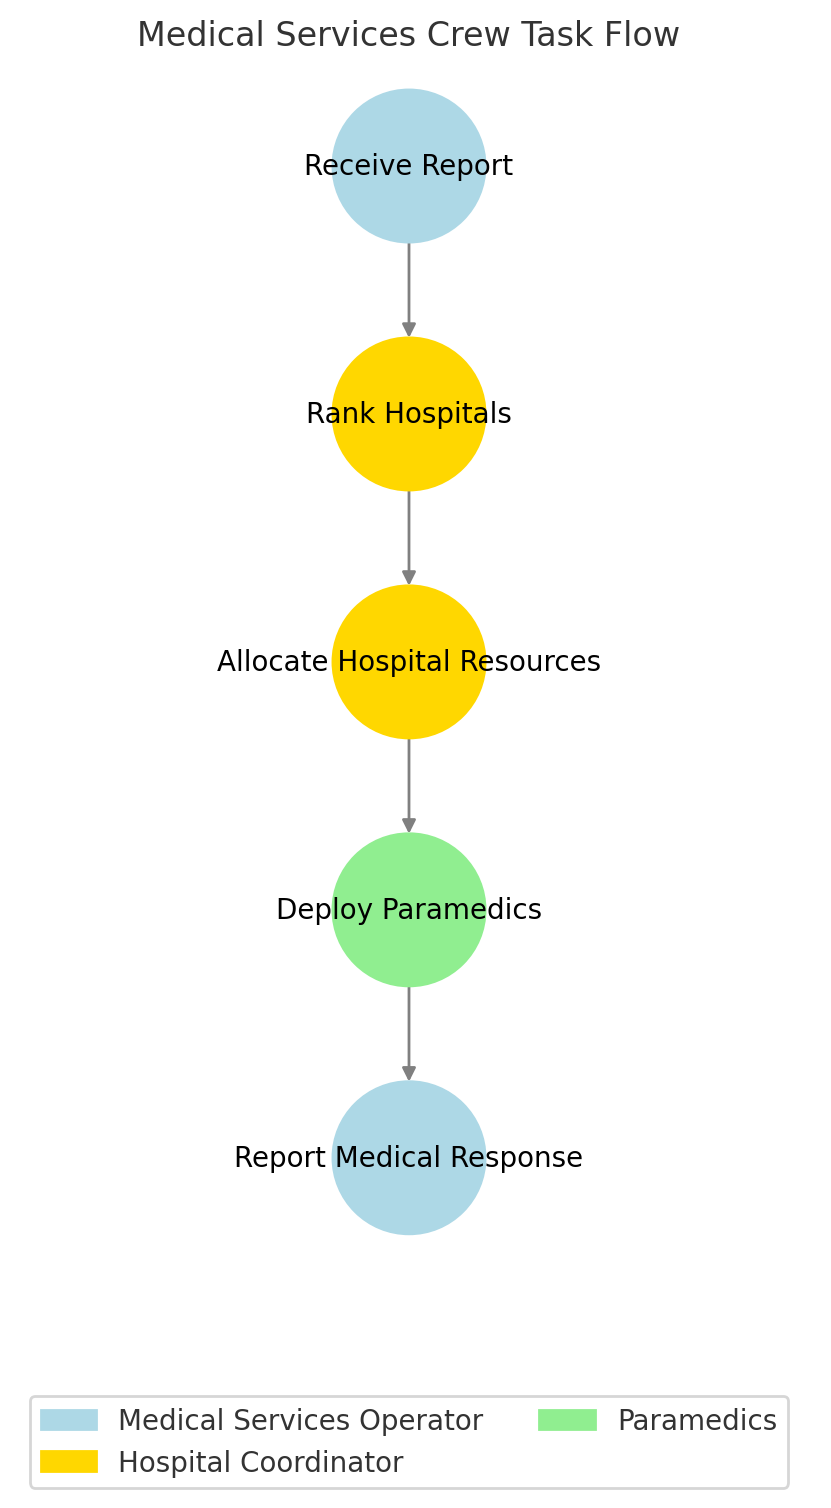
\includegraphics[height=0.6\textheight]{figures/Medical_Services_Crew_Flow.png}
	\caption{Sequential Process Flow of the Medical Services Crew with Agent Responsibilities}
	\label{fig:medical_services_flow}
\end{figure}
